\documentclass[pagesize]{scrartcl}

\usepackage[utf8]{inputenc}
\usepackage[T1]{fontenc}
\usepackage{enumitem}
\usepackage{amsmath}
\usepackage{amssymb}
\usepackage{amsthm}
\usepackage{graphicx}
\usepackage{tikz}
\usepackage{wrapfig}
\usepackage{animate}
%\usepackage{blindtext}
%\usepackage[bottom=5cm]{geometry}
%\pagestyle{empty} % no page numbering
\usepackage[hidelinks]{hyperref}




%verhindert einrückung bei neuem absatz
\setlength{\parindent}{0em} 

\vspace{-1cm}
\begin{document}
    \begin{center}
	\textsc{ \bfseries{\huge
			Poisson's equation\\ on an L-shaped domain}}
\\ 
	\vspace{2mm} Adéla Moravová, Barbara Präg \quad 27 January 2020

\end{center}

%\vspace{0.5cm}

%Investigate the regularity of the solution of Poisson's equation on an L-shaped domain. This is done by refining the discretization at the corner points. 

%What do you observe? How do these results compare to the results discussed in the exercises (for Poisson's equation on a square)?



\section{Poisson's equation}

\begin{minipage}{0.75\textwidth}
Consider the following elliptic problem with Dirichlet\\ boundary conditions 
\begin{align*}
	- \Delta u &= f \ \text{in} \ \Omega\\
	u &= 0 \ \text{on} \ \partial \Omega
\intertext{and its weak formulation with solution $u \in H_0^1(\Omega)$}
	\int_\Omega \nabla u \cdot \nabla v \ \text{d}x &= \int_\Omega f v \ \text{d}x \ \ \ \forall v \in H_0^1(\Omega),
\intertext{abbreviated as}
	a(u,v) &= (f,v) \ \ \forall v \in H_0^1(\Omega).
\end{align*}
\end{minipage}
\begin{minipage}{0.2\textwidth}
\centering
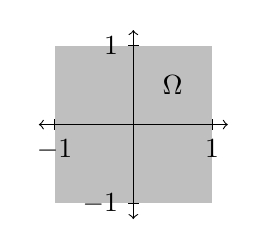
\begin{tikzpicture}[scale=1]
	%\draw (-1,-1) -- (-1,1) -- (1,1) -- (1,-1) -- (-1,-1);
 	\fill[fill = lightgray] (-1,-1) rectangle (1,1);

	\draw[<->] (-1.2,0) -- (1.2,0) coordinate (x axis);
 	\draw[<->] (0,-1.2) -- (0,1.2) coordinate (y axis);
 	
 	\foreach \x/\xtext in {-1/-1, 1/1}
 		\draw (\x,2pt) -- (\x,-2pt) node[anchor=north] {$\xtext$};
 	\foreach \y/\ytext in {-1/-1, 1/1}
 		\draw (2pt,\y) -- (-2pt,\y) node[anchor=east] {$\ytext$};
 		
 	\draw (0.5,0.5) node {$\Omega$};
 		
\end{tikzpicture}\\

vs.\\[0.3cm]

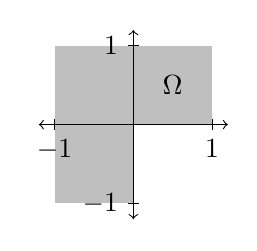
\begin{tikzpicture}[scale=1]
	%\draw (-1,-1) -- (-1,1) -- (1,1) -- (1,-1) -- (-1,-1);
 	\fill[fill = lightgray] (-1,-1) rectangle (1,1);
 	\fill[fill = white] (0,0) rectangle (1,-1);

	\draw[<->] (-1.2,0) -- (1.2,0) coordinate (x axis);
 	\draw[<->] (0,-1.2) -- (0,1.2) coordinate (y axis);
 	
 	\foreach \x/\xtext in {-1/-1, 1/1}
 		\draw (\x,2pt) -- (\x,-2pt) node[anchor=north] {$\xtext$};
 	\foreach \y/\ytext in {-1/-1, 1/1}
 		\draw (2pt,\y) -- (-2pt,\y) node[anchor=east] {$\ytext$};
 		
 	\draw (0.5,0.5) node {$\Omega$};
 		
\end{tikzpicture}
\end{minipage}


\flushleft

%\textbf{Reminder:} Sobolev spaces and their norms, $\Omega \subset \mathbb{R}^n$ open

%$H^k(\Omega) = \{u \in L^2(\Omega): D^\alpha u \in L^2(\Omega)$ for all $|a| \leq k\}$
%--> $H^0(\Omega) = L^2(\Omega)$

%$(u,v)_{H^k} = \sum_{|a| \leq k} \int_\Omega D^\alpha u \ D^\alpha v \ \text{d}x$

%$\|u\|_{H^k(\Omega)} = \sqrt{(u,u)_{H^k}}$

%$u \in H_0^1(\Omega)$ if $u \in H^1(\Omega)$ and "$u |_ { \partial \Omega} = 0$".\\[1cm]


\vspace{0.1cm}
\section{Shift theorems}

Let $\Omega$ be a convex polygonal domain in $\mathbb{R}^2$. If $u$ is the weak solution to our problem, then %%% "a" or "the" weak solution??
\begin{equation}
	\| u \|_{H^2} \leq C \| f \|_{H^0} \ \text{for} \ f \in H^0(\Omega) = L^2(\Omega).  \label{st}
\end{equation}\\[0.5ex]
% --> The solution is two times more "regular" than the right-hand side f. The elliptic differential operator "smoothes"

Similar shift theorems exist for \textbf{fractional-order Sobolev spaces} and $0 < s < s_0 < 1$ ($s_0$ is a constant depending on the domain):

\begin{equation*}
	H^s(\Omega) = W^{s,2}(\Omega) := \left\{ u \in L^2(\Omega): \frac{|u(x)-u(y)|}{|x-y|^{1+s}} \in  L^2(\Omega \times \Omega) \right\}
\end{equation*}
\begin{equation*}
	\|u\|_{H^s(\Omega)} = \|u\|_{W^{s,2}(\Omega)} := \left( \|u\|_{L^2(\Omega)}^2 + \iint_{\Omega \times \Omega} \left( \frac{|u(x)-u(y)|}{|x-y|^{1+s}} \right)^2  \text{d}x \ \text{d}y \right)^\frac{1}{2}
\end{equation*}

%%% H^s(\Omega) is constructed as the interpolation space between H^1(\Omega) and L^2(\Omega) with s-distance from L^2(\Omega).

Then, 
\begin{equation*}
	\|u\|_{H^{2+s}} \leq C \|f\|_{H^s} \ \text{for} \ f \in H^s(\Omega). \label{fo}
\end{equation*}\\[0.3cm]


For a smooth boundary $\partial \Omega$ it even holds that \begin{equation*}
	\|u\|_{H^{m+2}} \leq C \|f\|_{H^m} \ \text{for} \ f \in  H^m(\Omega) \ \text{and} \ m \in \mathbb{N}_0.
\end{equation*}

%Do we need to include m=-1? Should we then define it?

For $m=0$ and $m=1$ this is also true for a square. However, the regularity estimate never holds for non-convex polygonal domains like the L-shape.\\[0.5ex]

\begin{minipage}{0.4\textwidth}
	\includegraphics[scale=0.4]{sol37.png}
	%\animategraphics[autoresume, height=4cm]{15}{sol}{1}{15}
\end{minipage}
\begin{minipage}{0.5\textwidth}
	\includegraphics[scale=0.4]{derivatives2.png}
\end{minipage}
% Show that the derivative blows up at the kink.

%%% Comments on that...


% Show this...



\section{Finite element error}
Let $u$ be the weak solution of our elliptic problem, $\mathcal{T}_h$ a regular triangulation of a polygonal domain $\Omega$, $V_h = \{u \in C(\Omega) \cap H_0^1(\Omega): u|_T = \mathbb{P}^1 \ \forall\ T \in \mathcal{T}_h \}$ a piecewise linear finite element space and $u_h \in V_h$ the finite element solution,
Then,
% i.e., $ u_h \in V_h$ such that $a(u_h,v_h) = (f,v_h)$ for all $v_h \in V_h$,
\begin{equation*}
	\|u - u_h\|_{H^1(\Omega)} \leq C h \|u\|_{H^2(\Omega)}. \label{fee}
\end{equation*}

% The finite element error decreases with order h.

Under the assumption that $\Omega$ is convex and $u$ satisfies the shift theorem (\ref{st}), we also get an $L^2$ estimation for the finite element error:


%Let $z \in H_0^1(\Omega)$ be a solution of $a(z,v) = (u-u_h,v)$ for all  $v \in H_0^1(\Omega)$.

%For all $z_h \in V_h \subset H_0^1(\Omega)$, $a(u,z_h) = (f,z_h) = a(u_h,z_h)$. $\Rightarrow a(u-u_h,z_h) = 0$.\\
% $u-u_h \in H_0^1(\Omega)$, cf. \ref{fee}. and \ref{st}???

%\medskip
%Hence, $\|u-u_h\|_{L^2}^2 = (u-u_h,u-u_h) = a(z,u-u_h) = a(z-z_h,u-u_h) \leq$\\
%$\overset{\text{CS}}{\leq} \|\nabla(u-u_h)\|_{L^2} \cdot \|\nabla(z-z_h)\|_{L^2} \leq \|u-u_h\|_{H^1}  \cdot \|z-z_h\|_{H^1} \overset{(\ref{fee})}{\leq} Ch^2 \cdot \|u\|_{H^2} \cdot \|z\|_{H^2} \leq$\\
%$\overset{(\ref{st}) z}{\leq} \tilde{C}h^2\cdot \|u\|_{H^2} \cdot \|u-u_h\|_{H^0} = \tilde{C}h^2\cdot \|u\|_{H^2}\cdot \|u-u_h\|_{L^2}.$\\

%\medskip
%Therefore, $\|u-u_h\|_{L^2} \leq \tilde{C}h^2 \|u\|_{H^2}$.\\[2.5ex]

\begin{equation*}
	\|u-u_h\|_{L^2} \leq \tilde{C}h^2 \|u\|_{H^2}.
\end{equation*}\\[0.5ex]

If $\Omega$ is not convex, this inequality need not hold true.\\[0.8cm]



%Furthermore, under the assumption that (\ref{fo}) holds, 
%\begin{equation*}
%	\|u-u_h\|_{H^1} \leq Ch^{1+s} \|f\|_{H^s} \ \text{for} \ f \in H^s(\Omega).
%\end{equation*}\\[0.9cm]

%%% Add more possible results for the presentation...


\section{Refining the grid}

\begin{minipage}{0.5\textwidth}
Since the non-convexity at $(0,0)$ is causing the regularity problems in the L-shape (in comparison to the square), refining the grid close to this critical point should enhance the convergence of the finite element method.\\
\end{minipage}
\begin{minipage}{0.3\textwidth}
\centering
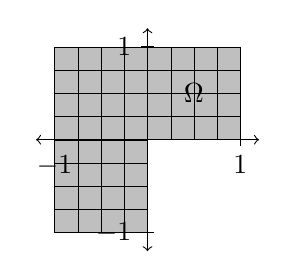
\begin{tikzpicture}[scale=1.18]
	%\draw (-1,-1) -- (-1,1) -- (1,1) -- (1,-1) -- (-1,-1);
 	\fill[fill = lightgray] (-1,-1) rectangle (1,1);
 	\draw[step=0.25cm, ultra thin] (-1,-1) grid (1,1);
	\fill[fill = white] (0,0) rectangle (1.1,-1.1);

	\draw[<->] (-1.2,0) -- (1.2,0) coordinate (x axis);
 	\draw[<->] (0,-1.2) -- (0,1.2) coordinate (y axis);
 	
 	\foreach \x/\xtext in {-1/-1, 1/1}
 		\draw (\x,2pt) -- (\x,-2pt) node[anchor=north] {$\xtext$};
 	\foreach \y/\ytext in {-1/-1, 1/1}
 		\draw (2pt,\y) -- (-2pt,\y) node[anchor=east] {$\ytext$};
 		
 	\draw (0.5,0.5) node {$\Omega$};
\end{tikzpicture}
\end{minipage}
\begin{minipage}{0.18\textwidth}
\centering
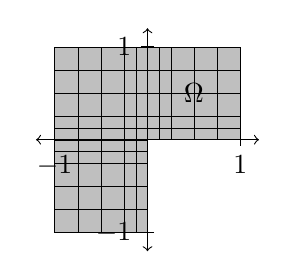
\begin{tikzpicture}[scale=1.18]
	%\draw (-1,-1) -- (-1,1) -- (1,1) -- (1,-1) -- (-1,-1);
 	\fill[fill = lightgray] (-1,-1) rectangle (1,1);
 	\draw[step=0.25cm, ultra thin] (-1,-1) grid (1,1);
 	\foreach \x in {0.125,-0.125}
 		\draw[ultra thin] (\x,1) -- (\x,-1);
 	\foreach \y in {0.125,-0.125}
 		\draw[ultra thin] (1,\y) -- (-1,\y);

 	\fill[fill = white] (0,0) rectangle (1.1,-1.1);

	\draw[<->] (-1.2,0) -- (1.2,0) coordinate (x axis);
 	\draw[<->] (0,-1.2) -- (0,1.2) coordinate (y axis);
 	
 	\foreach \x/\xtext in {-1/-1, 1/1}
 		\draw (\x,2pt) -- (\x,-2pt) node[anchor=north] {$\xtext$};
 	\foreach \y/\ytext in {-1/-1, 1/1}
 		\draw (2pt,\y) -- (-2pt,\y) node[anchor=east] {$\ytext$};
 		
 	\draw (0.5,0.5) node {$\Omega$};
 		
\end{tikzpicture}
\end{minipage}



\vspace{1.8cm}


\textbf{Literature:} \\
Demlow, Alan: \emph{Notes for Math 663. Chapter 1.} Spring 2016.\\
Bacuta, C., Bramble, J. H., Xu, Jinchao: \emph{Regularity estimates for elliptic boundary value problems with smooth data on polygonal domains.} January 8, 2003.

%Plot von den Verfassern erstellt.




\end{document}
